\documentclass[10pt]{mypackage}

% sans serif font:
%\usepackage{cmbright,sfmath,bbold}
%\renewcommand{\mathcal}{\mathtt}

%Euler:
\usepackage{newpxtext,eulerpx,eucal,eufrak}
\renewcommand*{\mathbb}[1]{\varmathbb{#1}}
\renewcommand*{\hbar}{\hslash}

\usepackage{homework}

\pagestyle{fancy} %better headers
\fancyhf{}
\rhead{Avinash Iyer}
\lhead{Assignment 1}

\setcounter{secnumdepth}{0}

\begin{document}
\RaggedRight
\renewcommand{\arraystretch}{1.5}
\begin{solution}[18.1]\hfill
  \begin{enumerate}[(a)]
    \item The function $f(z) = z^n$ is analytic on $\C$.
    \item The functions $f(z) = \sin(z)$ and $f(z) = \cos(z)$ are analytic on $\C$, while $f(z)= \tan(z)$ is analytic everywhere except for singularities at $n\pi/2$.
    \item The function $f(z) = \left\vert z \right\vert$ is analytic nowhere.
    \item The function $f(z) = \frac{z-i}{z+1}$ is analytic everywhere except for $z = -1$.
    \item The function $f(z) = \frac{z^2 + 1}{z}$ is analytic everywhere except for $z = 0$.
    \item The function $f(z) = \frac{p_n(z)}{q_m(z)}$ is analytic everywhere except for the roots of $q$.
    \item The function $x^2 + y^2$ is analytic nowhere.
    \item The function $e^z$ is analytic on $\C$.
    \item The function $e^{-iy}$ is analytic nowhere.
    \item The function $\ln\left(z\right)$ is analytic everywhere except for $(-\infty,0]$.
  \end{enumerate}
\end{solution}
\begin{solution}[18.2]
  Let $w(z) = u\left(x,y\right) + iv\left(x,y\right)$. Then,
  \begin{align*}
    i\pd{}{x}\left(w(x + iy)\right) - \pd{}{y}\left(w\left(x+ iy\right)\right) &= i \pd{}{x}\left(u\left(x,y\right) + iv\left(x,y\right)\right) - \pd{}{y}\left(u\left(x,y\right) + iv\left(x,y\right)\right)\\
                                                                               &= i\left(\pd{u}{x} - \pd{v}{y}\right) - \left(\pd{u}{y} + \pd{v}{x}\right).
  \end{align*}
  Thus, we get
  \begin{align*}
    \pd{u}{x} &= \pd{v}{y}\\
    \pd{u}{y} &= -\pd{v}{x}.
  \end{align*}
\end{solution}
\begin{solution}[18.4]
  We see that, when we have $w(z) = u(x,y) + iv(x,y)$, that
  \begin{align*}
    \nabla u &= \begin{pmatrix}\diff{u}{x} \\ \diff{u}{y}\end{pmatrix}\\
    \nabla v &= \begin{pmatrix} \diff{v}{x} \\ \diff{v}{y}\end{pmatrix}.
  \end{align*}
  We note that curves of constant $u$ and $v$ are orthogonal if and only if the normal vectors are orthogonal, meaning
  \begin{align*}
    \left( \nabla u \right)\cdot \left( \nabla v \right) &= \diff{u}{x}\diff{v}{x} + \diff{u}{y} \diff{v}{y}\\
                                                         &= \diff{v}{y}\diff{v}{x} - \diff{v}{x}\diff{v}{y}\\
                                                         &= 0.
  \end{align*}
\end{solution}
\begin{solution}[18.5]
  We see that
  \begin{align*}
    \pd{^2u}{x^2} &= \pd{v}{x\partial y}\\
    \pd{^2 u}{y^2} &= -\pd{v}{x\partial y},
  \end{align*}
  so 
  \begin{align*}
    \pd{^2u}{x^2} + \pd{^2u}{y^2} &= 0.
  \end{align*}
  Symmetrically, we also have that $v$ satisfies Laplace's equation.
\end{solution}
\begin{solution}[18.6]\hfill
  \begin{enumerate}[(a)]
    \item We start by writing everything in terms of $z$, so we have $w(z) = u(z) + iv(z)$. Since $w$ is complex-differentiable, by linearity we have
      \begin{align*}
        w'(z) &= \diff{u}{z} + i\diff{v}{z}.
        \intertext{We write $z = x + iy$, or $x = \frac{z + \overline{z}}{2},y = \frac{z - \overline{z}}{2i}$.}
              &= \pd{u}{x}\pd{x}{z} + \pd{u}{y}\pd{y}{z} + \pd{v}{x}\pd{x}{z} + \pd{v}{y}\pd{y}{z}\\
              &= \frac{1}{2}\left( \pd{u}{x} + \pd{v}{y} + i\left( \pd{v}{x} - \pd{u}{y} \right)  \right).
      \end{align*}
    \item We have that
      \begin{align*}
        \pd{u}{x} + i\pd{v}{x} &= \pd{u}{y} + i\pd{v}{y}\\
                               &= \frac{1}{2}\left( \pd{u}{x} + \pd{v}{y} + i\left( \pd{v}{x} - \pd{u}{y} \right) \right).
      \end{align*}
      Thus, by tedious algebraic manipulations heavily prone to error, we recover the Cauchy--Riemann equations:
      \begin{align*}
        \pd{u}{x} &= \pd{v}{y}\\
        \pd{u}{y} &= -\pd{v}{x}.
      \end{align*}
  \end{enumerate}
\end{solution}
\begin{solution}[18.7]
  We find that
  \begin{align*}
    \diff{w}{z} &= \pd{u}{x} + i\pd{v}{x}\\
                &= 1\\
                &= \pd{u}{y} + i\pd{v}{y}\\
                &= -i.
  \end{align*}
  Since these derivatives are path-dependent, we have that $w(z) = \overline{z}$ is not differentiable.
\end{solution}
\begin{solution}[18.11]
  Using the scale factors, we recall that $d\mathbf{x} = dr + rd\phi$, so the derivatives with respect to $\phi$ pick up a scale term of $\frac{1}{r}$. This yields our desired Cauchy--Riemann equations in polar form:
  \begin{align*}
    \diff{u}{r} &= \frac{1}{r}\diff{v}{\phi}\\
    \frac{1}{r}\diff{u}{\phi} &= - \diff{v}{r}. 
  \end{align*}
\end{solution}
\begin{solution}[18.14]
  We know that $\frac{1}{z^m}$ is defined for all $z\in \C\cup\set{\infty}\setminus \set{0}$, so we only need to show that if $ z\neq 0 $, then $\frac{1}{z^m}$ admits a derivative. We see that
  \begin{align*}
    \diff{}{z}\left( \frac{1}{z^m} \right) &= \frac{-m}{z^{m+1}},
  \end{align*}
  which is yet again defined for all $z\neq 0$, so $\frac{1}{z^m}$ is analytic on its domain.
\end{solution}
\begin{solution}[18.15]
  \begin{align*}
    \oint_{C} \frac{1}{z^n}\:dz  &= \oint_{C}\left( r^{-n}e^{-in\varphi} \right)ire^{i\varphi}\:d\varphi\\
                                 &= \frac{1}{r^{n-1}}\int_{0}^{2\pi}ie^{-i\left( n-1 \right)\varphi}\:d\varphi\\
                                 &= 0.
  \end{align*}
\end{solution}
\begin{solution}[18.18]\hfill
  \begin{enumerate}[(a)]
    \item \hfill
      \begin{center}
        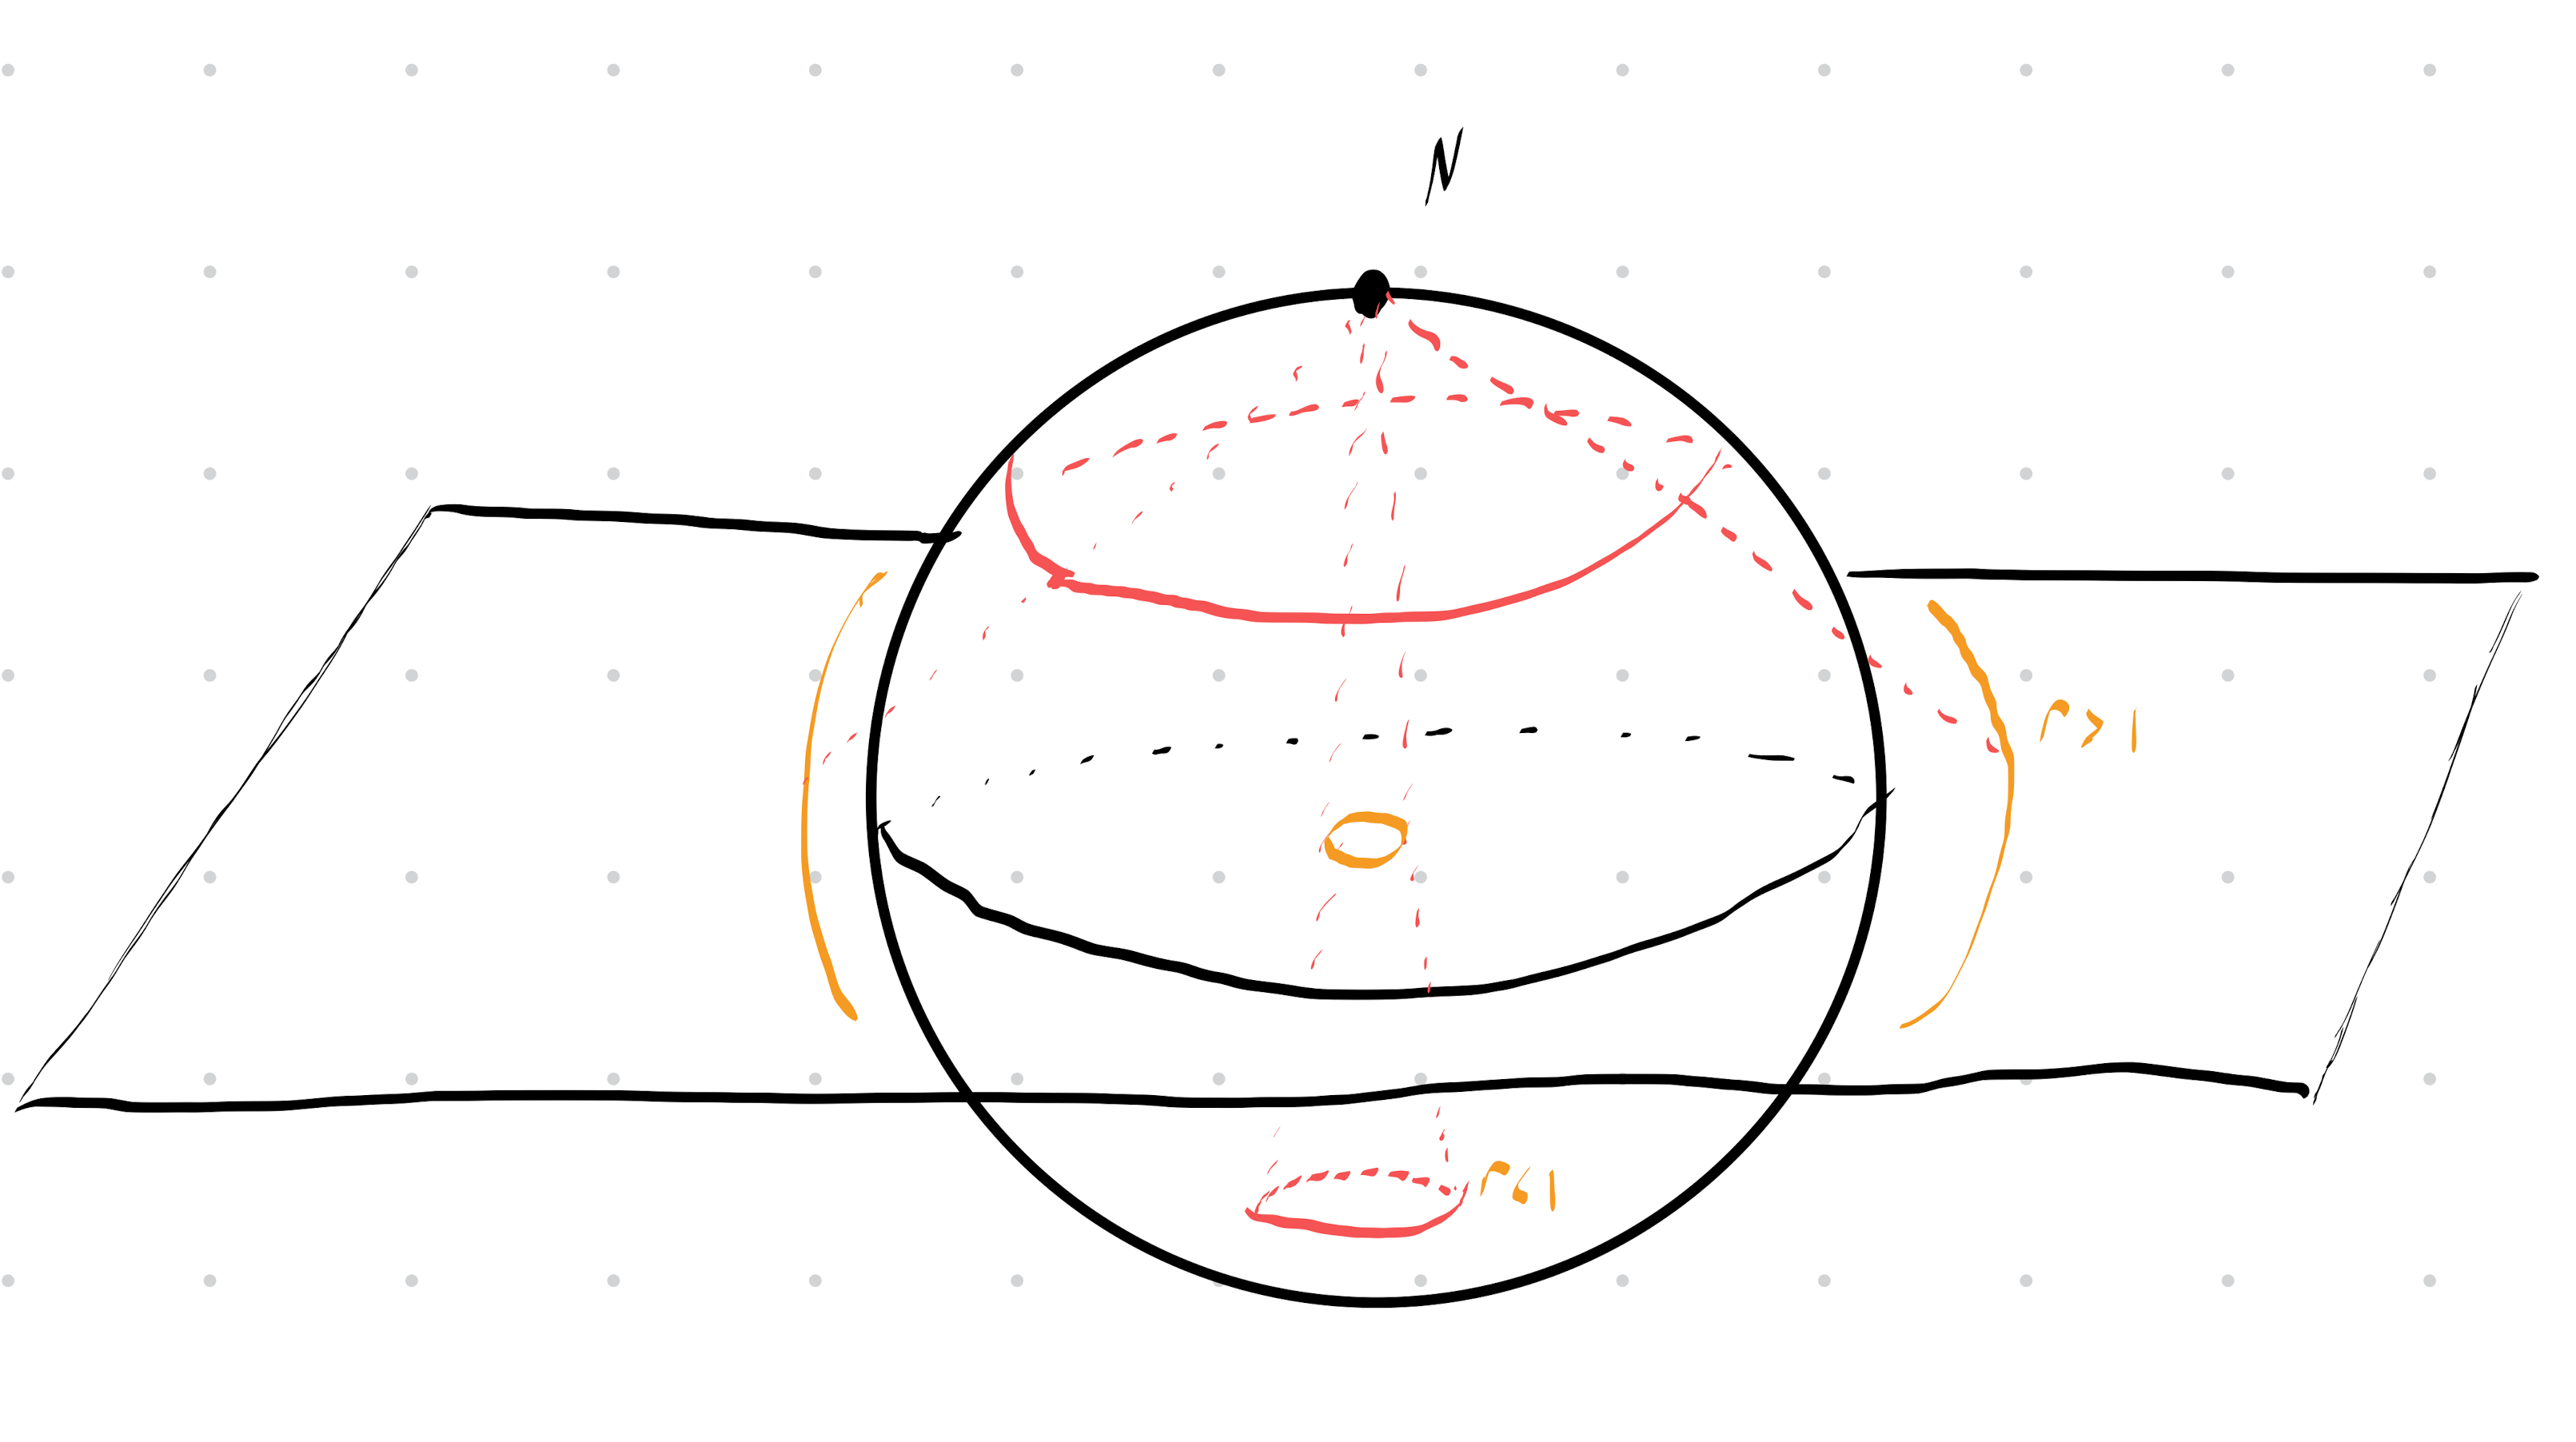
\includegraphics[width=10cm]{images/18_18_a.png}
      \end{center}
    \item \hfill
      \begin{center}
        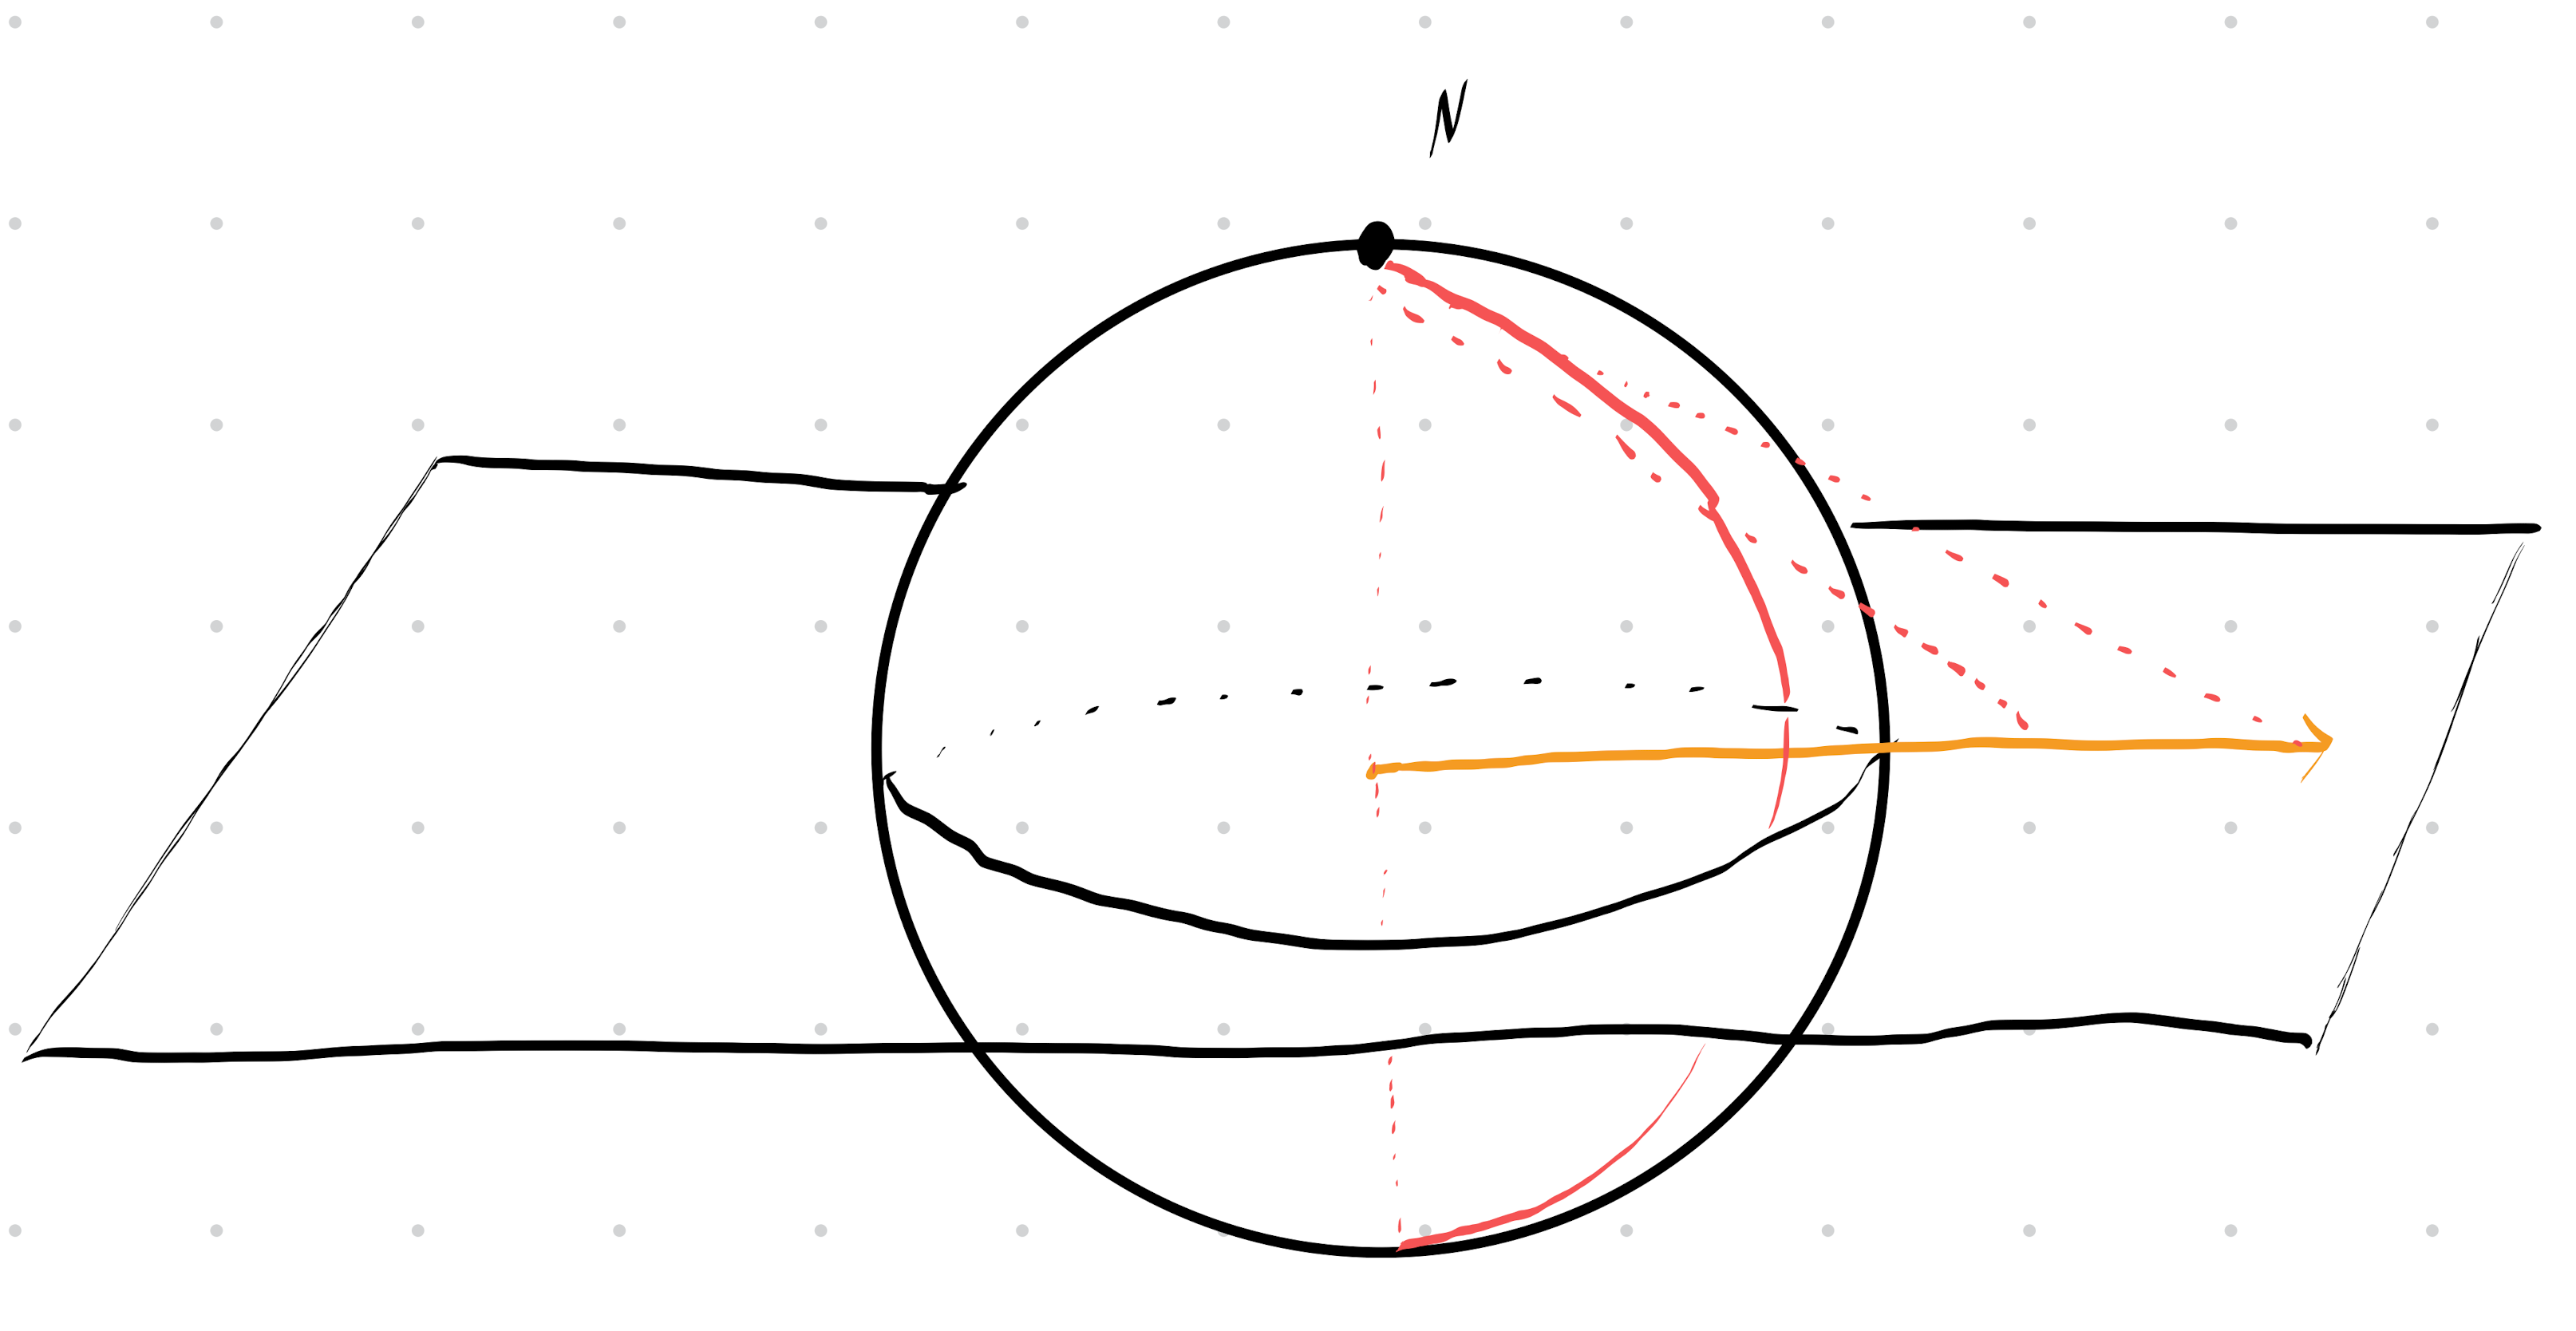
\includegraphics[width=10cm]{images/18_18_b.png}
      \end{center}
    \item \hfill
      \begin{center}
        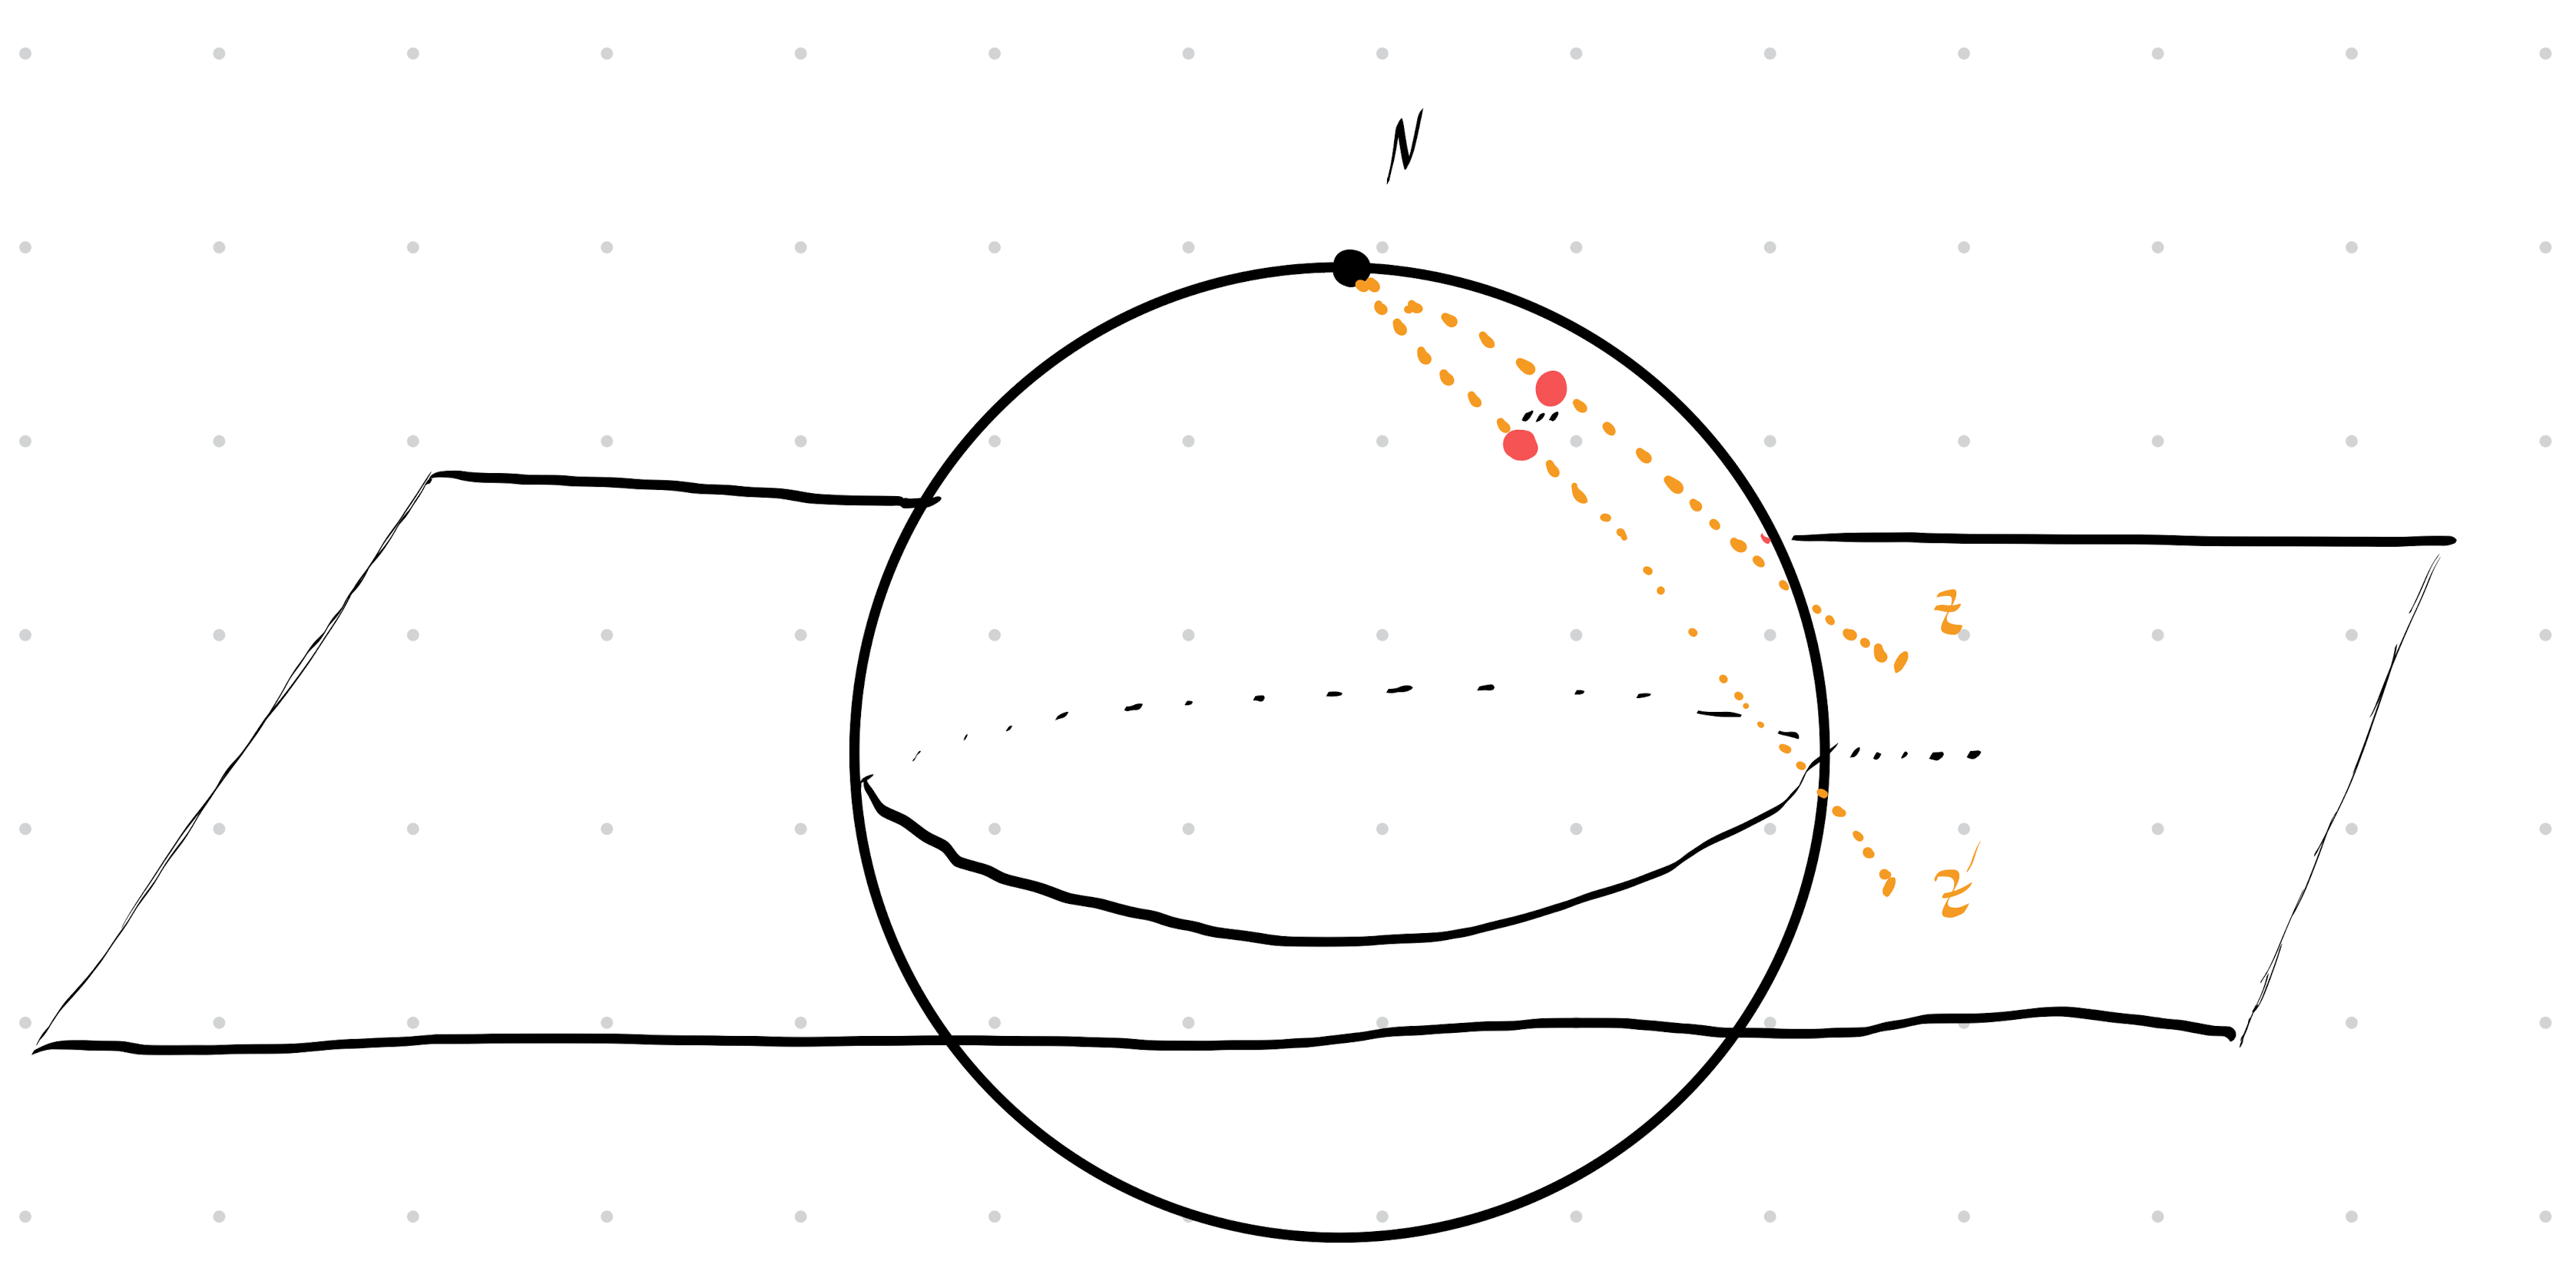
\includegraphics[width=10cm]{images/18_18_c.png}
      \end{center}
    \item \hfill
      \begin{center}
        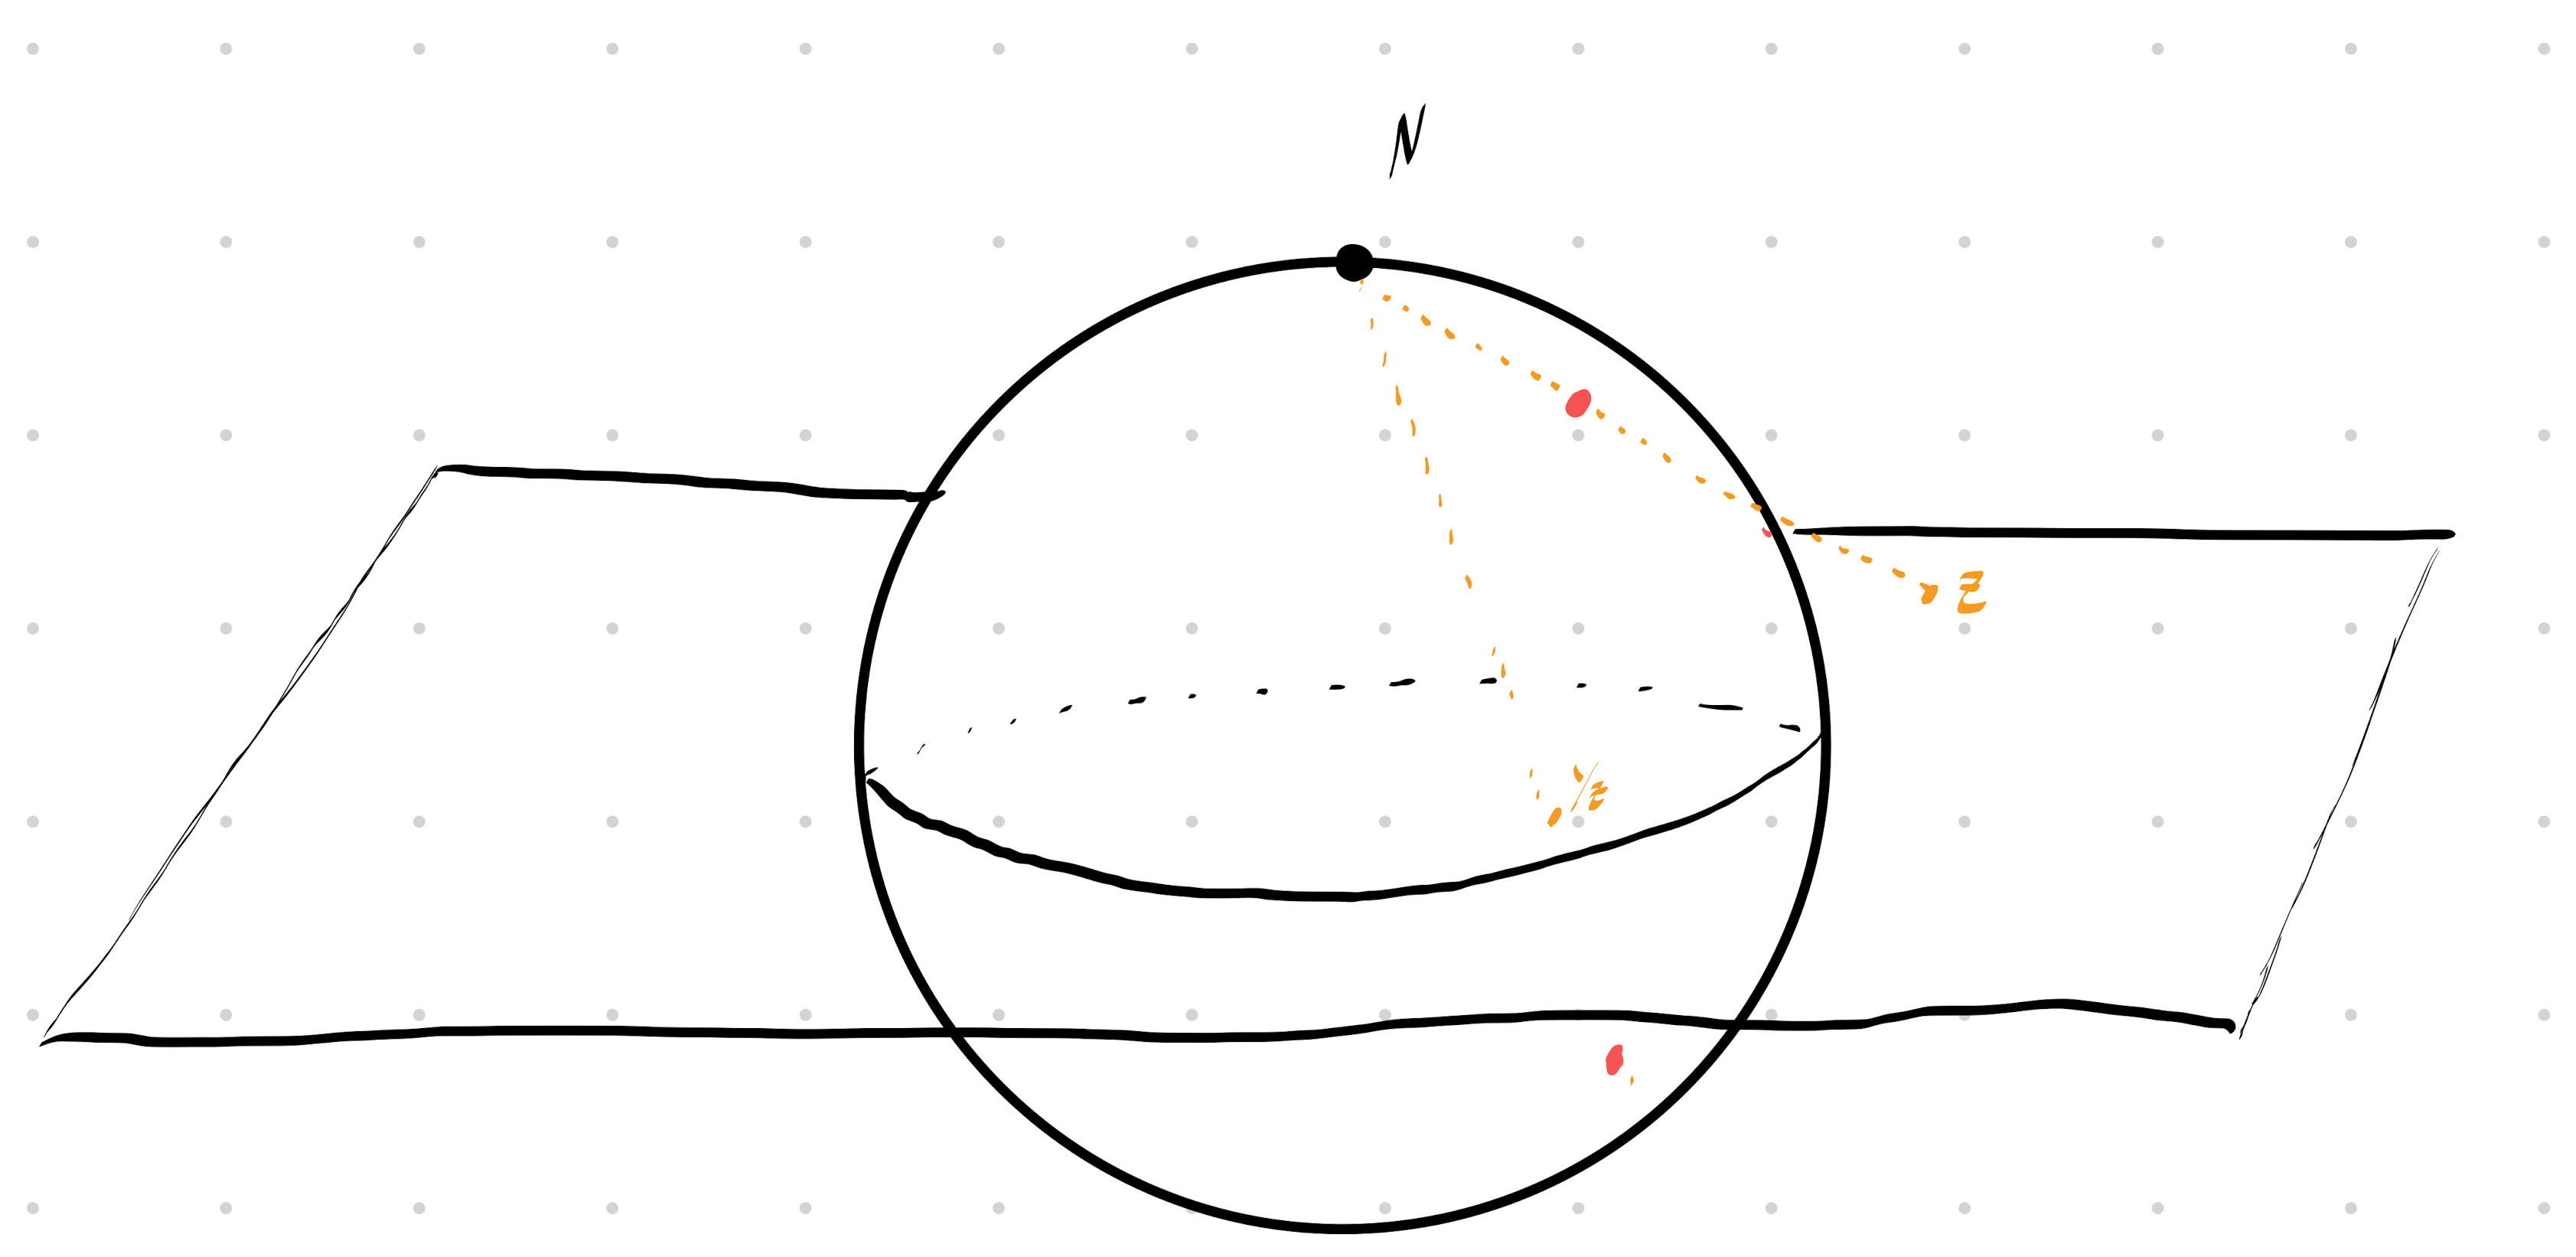
\includegraphics[width=10cm]{images/18_18_d.png}
      \end{center}
    \item \hfill
      \begin{center}
        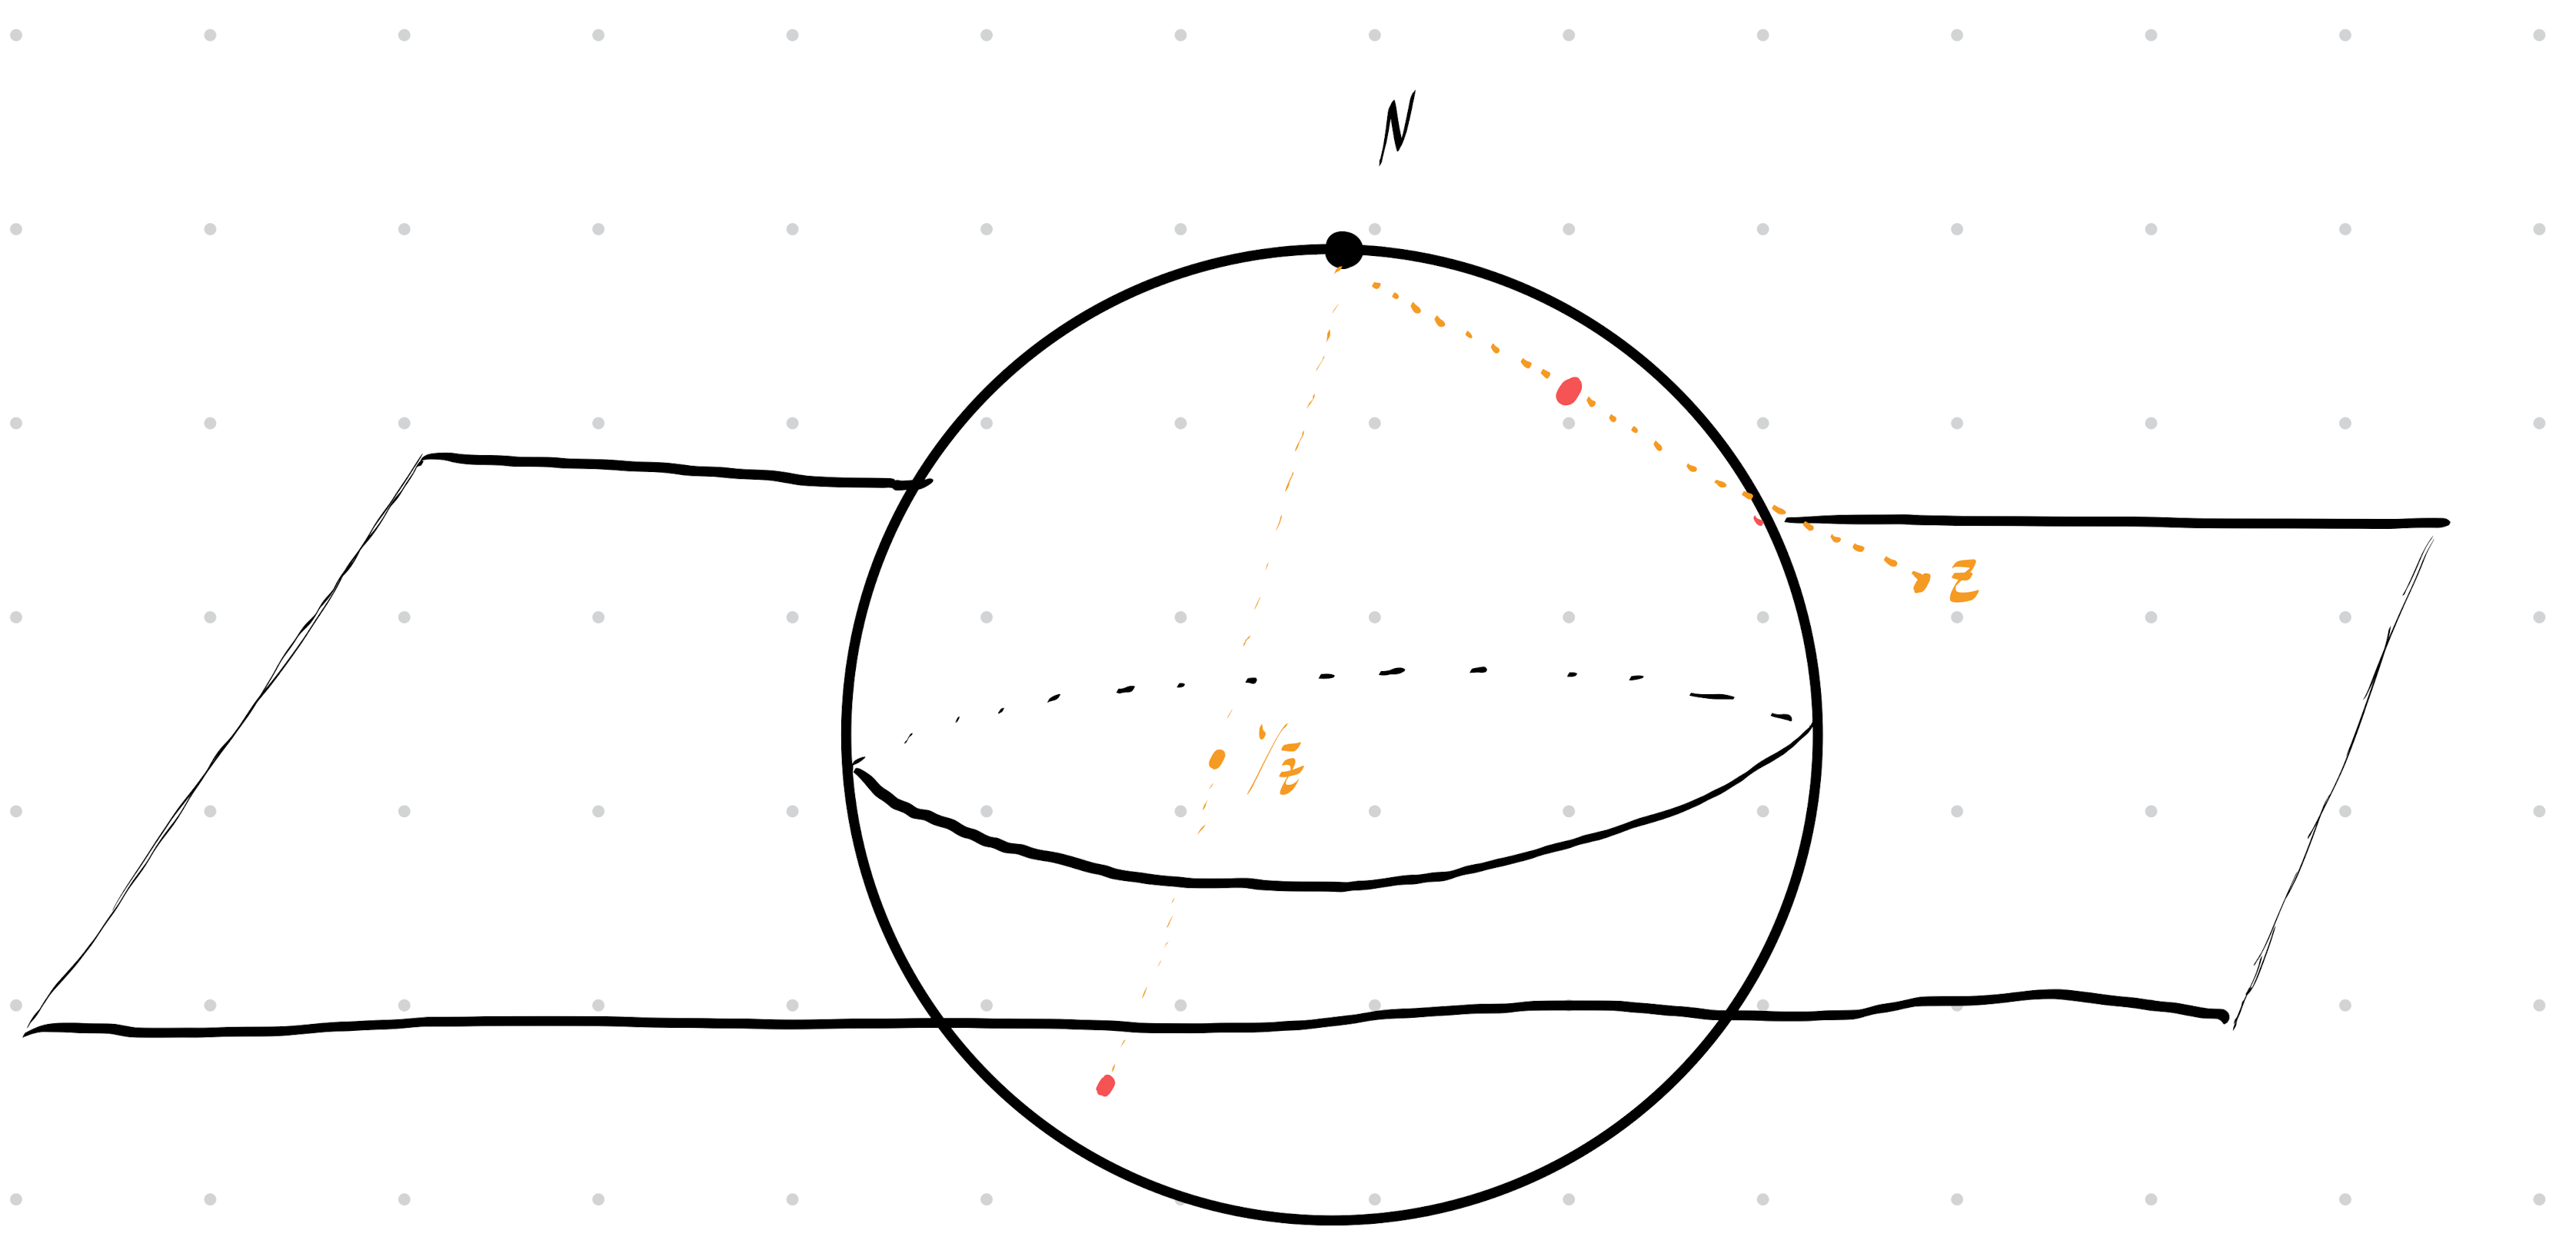
\includegraphics[width=10cm]{images/18_18_e.png}
      \end{center}
  \end{enumerate}
\end{solution}
\end{document}
